\documentclass[a4paper,12pt]{article}

\usepackage{geometry}
\usepackage{polski}
\usepackage{amsmath}
\usepackage{makecell}
\usepackage{ragged2e}
\usepackage{hyperref}
\usepackage{array}
\usepackage{pdfpages}
\usepackage{xparse}
\NewDocumentCommand{\DIV}{om}{%
  \IfValueT{#1}{\setcounter{#2}{\numexpr#1-1\relax}}%
  \csname #2\endcsname
}
\graphicspath{ {./} }

\hypersetup{
	colorlinks=true,
	linkcolor=black,
	filecolor=magenta,
	urlcolor=blue,
	citecolor=black
}

\urlstyle{same}

\geometry{
 a4paper,
 total={170mm,257mm},
 left=20mm,
 top=20mm,
 }
 
\pagenumbering{arabic}

\begin{document}
\begin{justify}

\begin{center}
\begin{scriptsize}
\begin{tabular}{ |m{2.5cm}|l|l|l|l|l| }
	\hline
	\makecell{Wydział: \\ FiIS} & \multicolumn{2}{|l|}{\makecell{Imię i nazwisko: \\ 1. Piotr Moszkowicz \\ 2. Wiktor Jasiński}}  & \makecell{Rok: \\ Drugi} & \makecell{Grupa: \\ PN 14:40} & \makecell{Zespół: \\ 1} \\
	\hline
	\textbf{PRACOWNIA FIZYCZNA WFiIS AGH} & \multicolumn{4}{|l|}{\makecell{Temat: Modelowanie pola elektrycznego }}  & \makecell{Nr ćwiczenia: \\ 31} \\
	\hline
	\makecell{Data wykonania: \\ 18.03.2019} & \makecell{Data oddania: \\ 25.03.2019} & \makecell{Zwrot do popr. \\ \,} & \makecell{Data oddania \\ \,} & \makecell{Data zaliczenia \\ \,} & \makecell{OCENA \\ \,} \\
	\hline
\end{tabular}
\end{scriptsize}

\vspace{2cm}

\begin{Large}
\textbf{Ćwiczenie nr 31: Modelowanie pola elektrycznego}
\end{Large}

\end{center}

\vspace{0.5cm}
\textbf{Cel ćwiczenia:} \\
\indent Wyznaczenie linii ekwipotencjalnych i wektorów natężenia pola elektrycznego na płaszczyźnie dla różnych konfiguracji elektrod. \cite{instrukcja} 
\end{justify}

\newpage

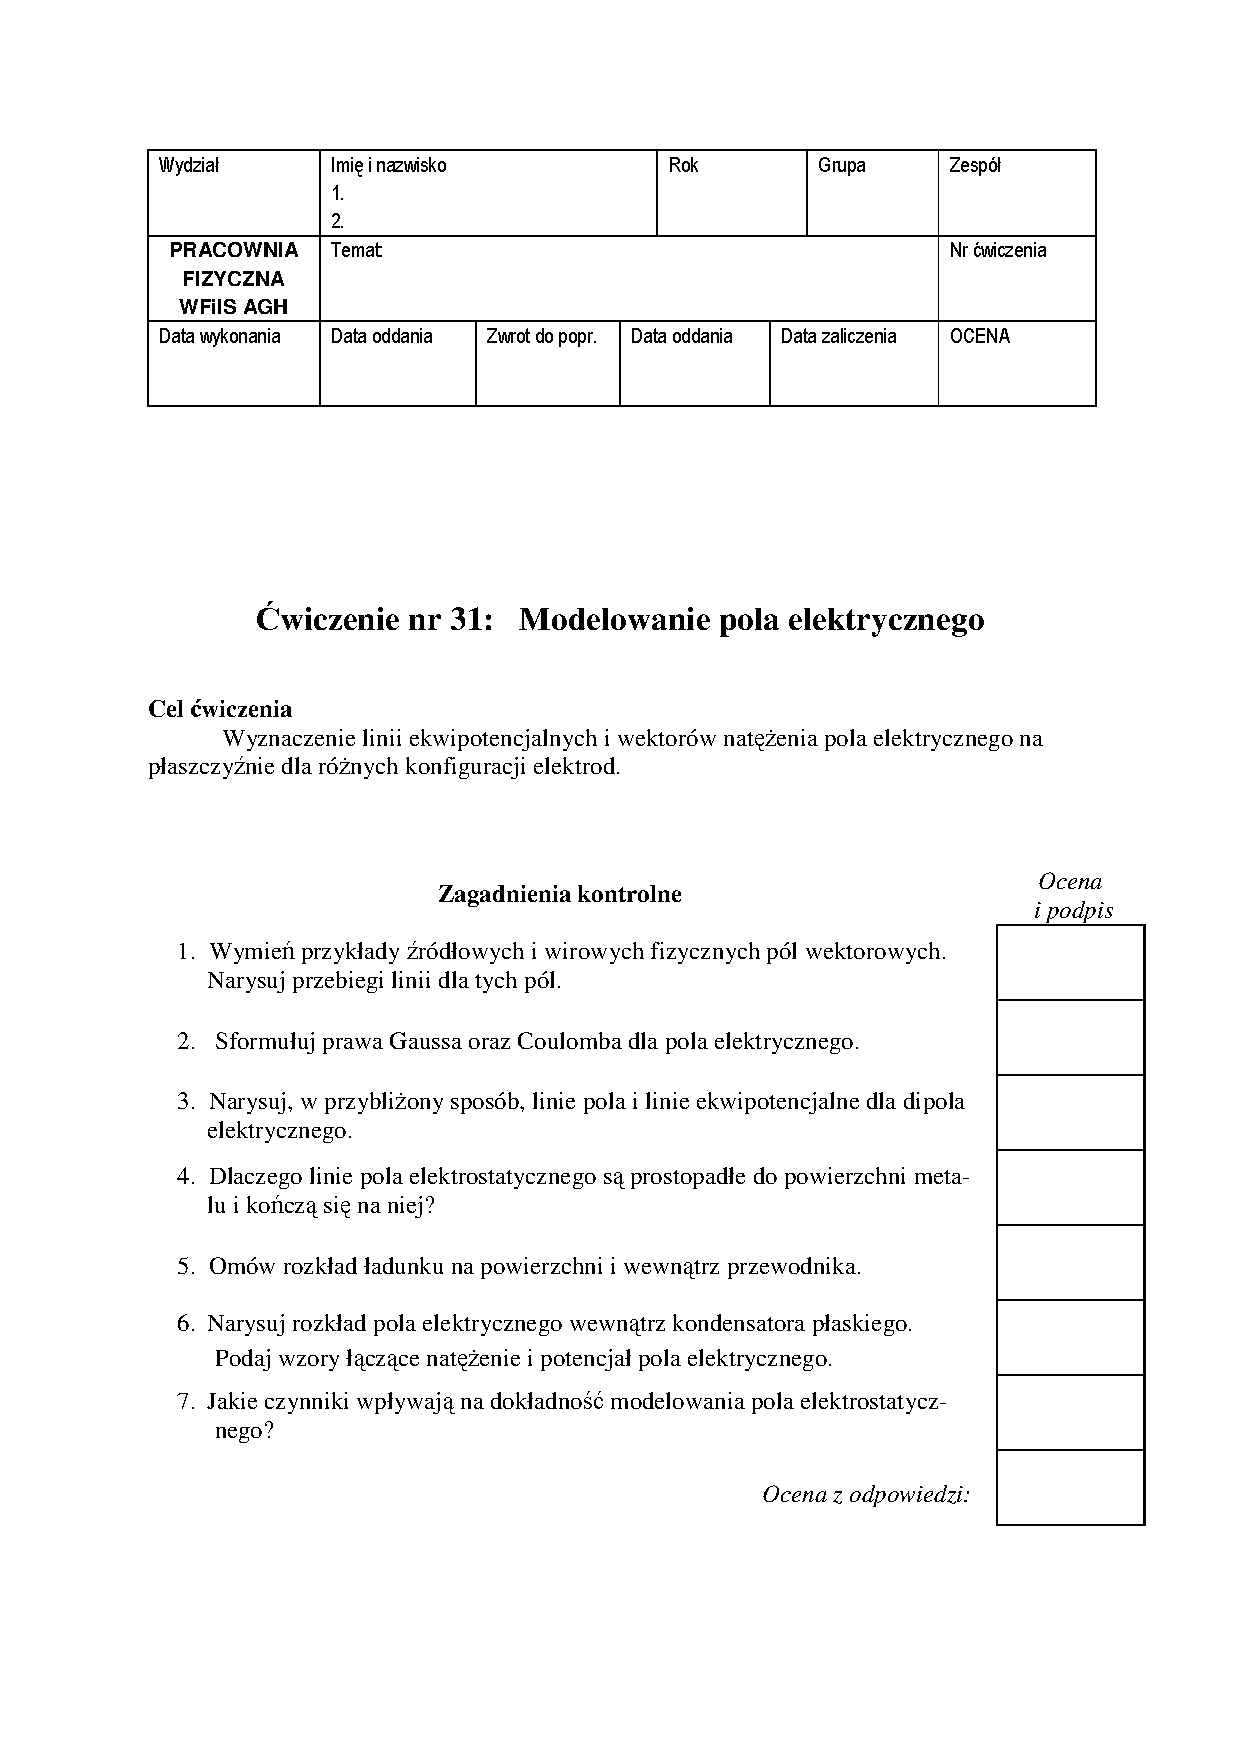
\includepdf[page={2,3}]{31_wykon}

\begin{justify}

\DIV[3]{section}{Wstęp teoretyczny}
\label{theory}

\subsection{Pole elektryczne}

Pole wektorowe określające w każdym punkcie siłę działającą na jednostkowy, spoczywający ładunek elektryczny. Pole elektryczne wytwarzane jest przez ładunki elektryczne oraz zmieniające się pole magnetyczne. \cite{pe} 

\subsection{Potencjał elektryczny}

Potencjałem elektrycznym $\varphi$  w dowolnym punkcie P stałego pola elektrycznego nazywa się stosunek pracy W wykonanej przez siłę elektryczną przy przenoszeniu ładunku q z tego punktu do nieskończoności, do wartości tego ładunku: \\
$\varphi _{{P}}={\frac  {W_{{P\rightarrow \infty }}}{q}}$

Jednostką potencjału jest 1 V (wolt) równy 1 J / 1 C (dżulowi na kulomb). \cite{pote}

\subsection{Natężenie pola elektrycznego}

Natężenie pola elektrycznego – wektorowa wielkość fizyczna charakteryzująca pole elektryczne.

Natężenie pola elektrycznego jest równe sile działającej na jednostkowy dodatni ładunek próbny, co matematycznie wyraża się jako stosunek siły $\vec  {F}$, z jaką pole elektryczne działa na ładunek elektryczny, do wartości q tego ładunku. \\

$\vec {E}=\frac {\vec {F}}{q}$ \\

Ładunek próbny oznacza ładunek na tyle mały, że nie wpływa on znacząco na rozkład ładunków w badanym obszarze i tym samym nie zmienia pola elektrycznego w badanym punkcie.
Jednostką natężenia pola elektrycznego jest niuton na kulomb \\

$ \left[{\vec {E}}\right]={\frac {\operatorname {N} }{\operatorname {C} }}$ \\
co jest równoważne woltowi na metr \\

$\left[{\vec {E}}\right]={\frac {\operatorname {V} }{\operatorname {m} }}$ \\

Natężenie pola elektrycznego obrazuje się stosując techniki używane do obrazowania pól wektorowych, rysując linie sił pola (linie styczne do wektora siły działającej na ładunek dodatni), których gęstość odzwierciedla lokalne natężenie pola. \cite{npe}

\subsection{Kondensator płaski}

Element elektryczny (elektroniczny), zbudowany z dwóch przewodników (okładek) rozdzielonych dielektrykiem. \cite{konder}

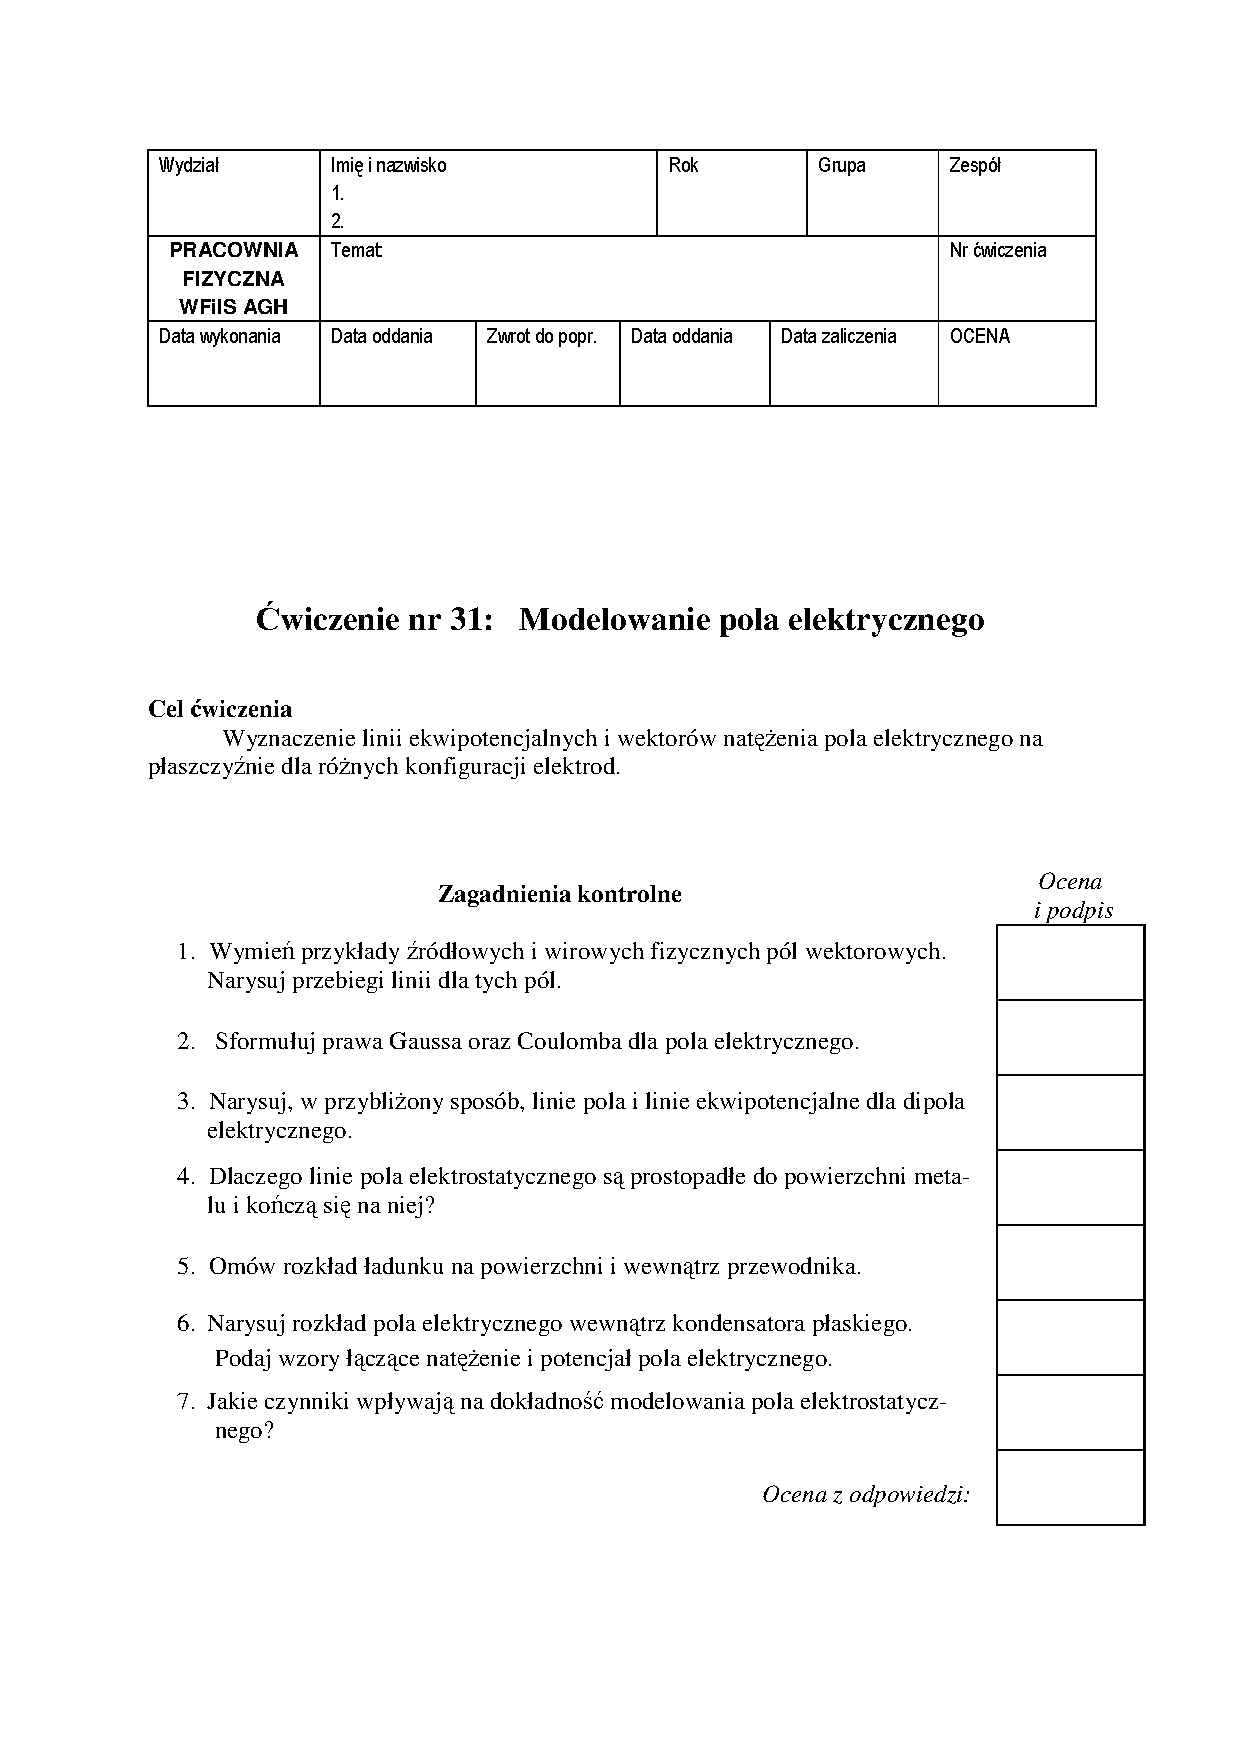
\includepdf[page={8}]{31_wykon}

\DIV[5]{section}{Aparatura pomiarowa}

Przy tym doświadczeniu będziemy korzystać z poniższych przedmiotów:
\begin{itemize}
\item Zasilacz
\item Kondensator płaski
\item Sonda do pomiaru napięcia
\item Miernik napięcia
\end{itemize}

\section{Wyniki pomiarów}

\subsection{Wyniki pomiarów i obliczeń dla płaskiego układu elektrod}

\begin{center}
\begin{tabular}{ |c|c|c|c|c|c|c| }
\hline
L.p. & x [mm] & $V_{a}$ [V] & $V_{b}$ [V] & $V_{c}$ [V] & $V_{dosw} = \frac{V_{a} + V_{b} + V_{c}}{3} $ [V] & $V_{teor}$ [V] \\
\hline
1 & 3 & 1.154 & 1.195 & 1.021 & 1.123 & 1.360 \\
\hline
2 & 5 & 2.029 & 2.089 & 2.363 & 2.160 & 2.270 \\
\hline
3 & 7 & 3.002 & 3.047 & 3.015 & 3.021 & 3.180 \\
\hline
4 & 9 & 3.996 & 4.023 & 3.825 & 3.948 & 4.090 \\
\hline
5 & 11 & 4.918 & 4.895 & 5.073 & 4.962 & 5.000 \\
\hline
6 & 13 & 5.871 & 5.836 & 5.801 & 5.836 & 5.910 \\
\hline
7 & 15 & 6.885 & 6.739 & 6.692 & 6.772 & 6.820 \\
\hline
8 & 17 & 7.849 & 7.818 & 7.701 & 7.789 & 7.730 \\
\hline
9 & 19 & 8.870 & 8.791 & 8.582 & 8.747 & 8.690 \\
\hline
\end{tabular}
\end{center}

\subsection{Wyniki pomiarów potrzebnych do wyliczenia potencjałów w punktach}

\paragraph{Na następnej stronie widać spis punktów na rysunku, których pomiary zostały wykonane. Na kolejnej stronie ukazane są wyniki tychże pomiarów.}

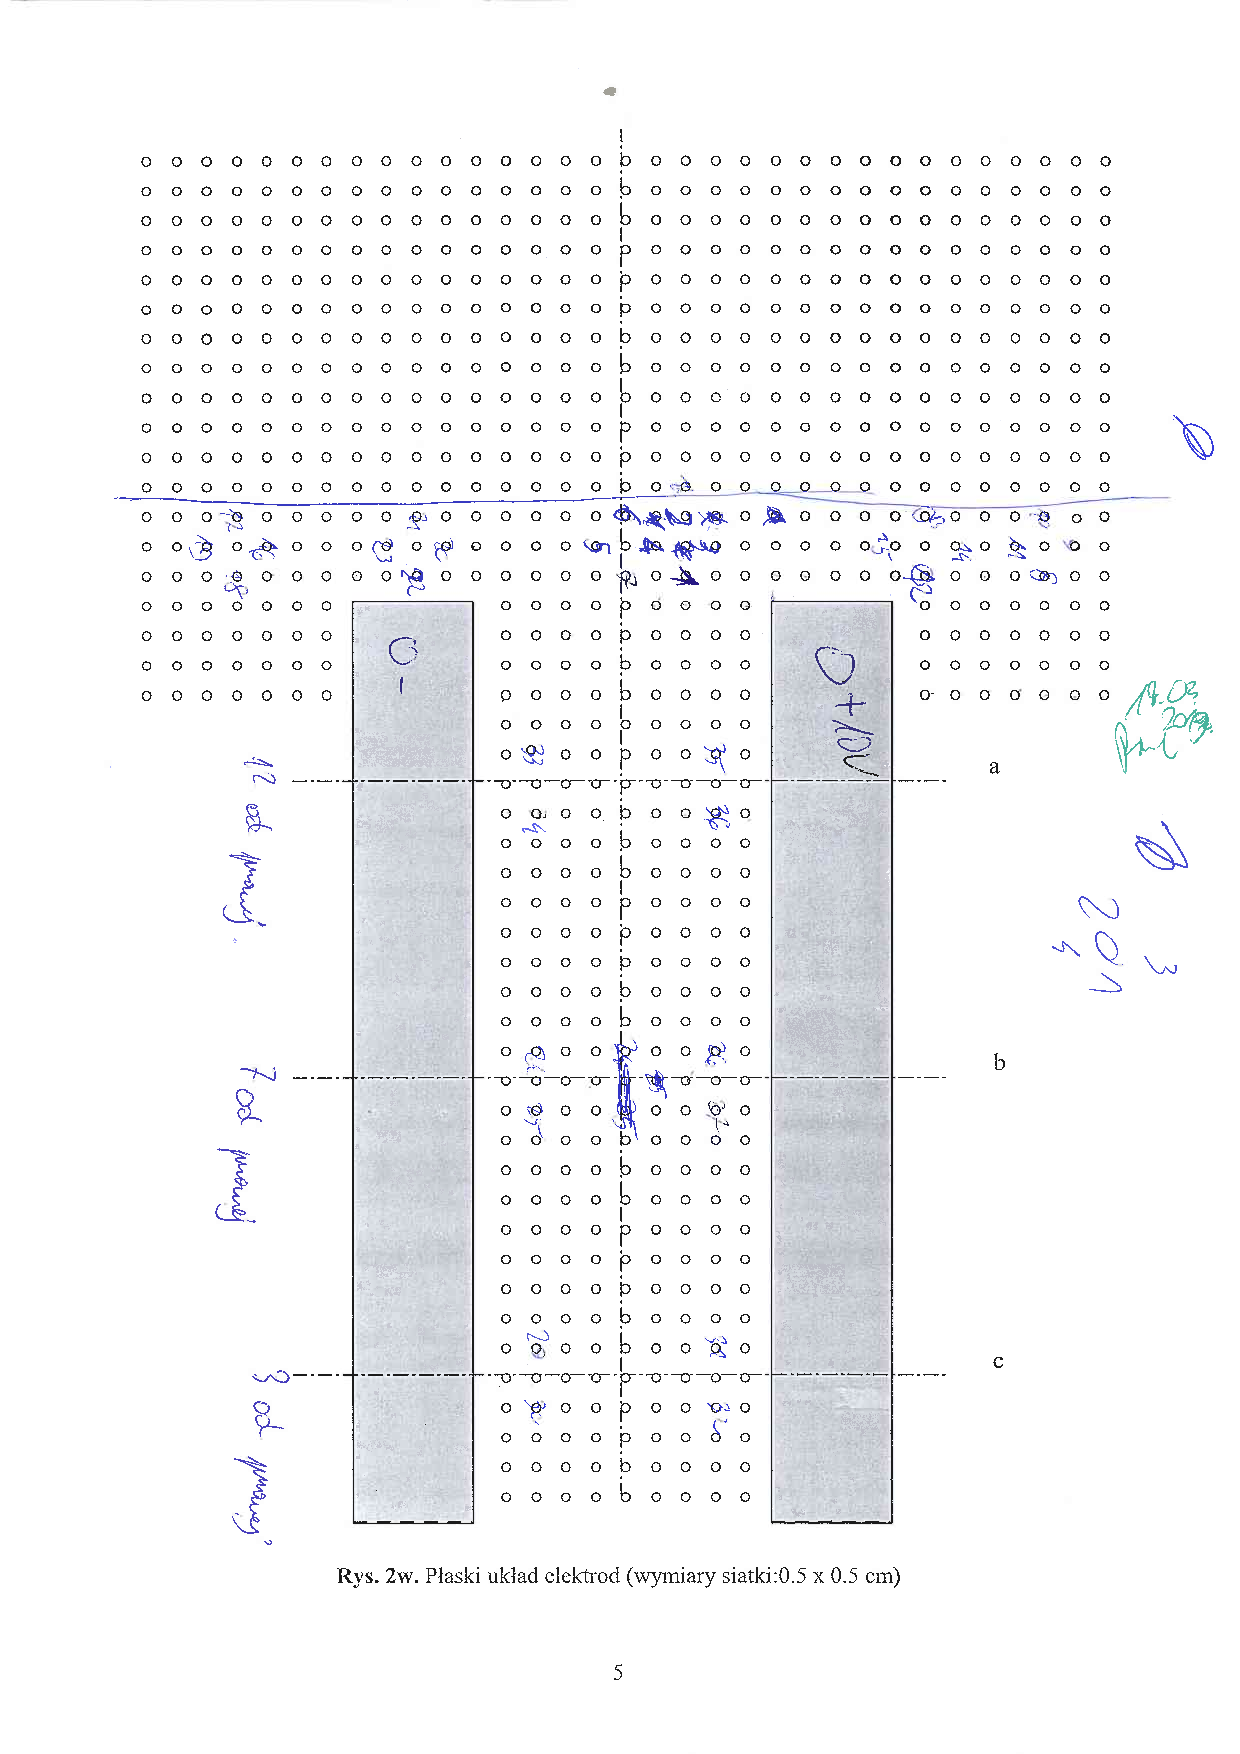
\includepdf[page={1}]{scan}

\begin{center}
\begin{tabular}{ |c|c| }
\hline
L.p. z rysunku & $V$ [V] \\
\hline
1 & 6.305 \\
\hline
2 & 5.903 \\
\hline
3 & 6.680 \\
\hline
4 & 5.569 \\
\hline
5 & 4.235 \\
\hline
6 & 4.915 \\
\hline
7 & 5.085 \\
\hline
8 & 9.065 \\
\hline
9 & 8.730 \\
\hline
10 & 8.740 \\
\hline
11 & 8.872 \\
\hline
12 & 9.172 \\
\hline
13 & 8.266 \\
\hline
14 & 8.612 \\
\hline
15 & 8.599 \\
\hline
16 & 1.102 \\
\hline
17 & 1.304 \\
\hline
18 & 0.740 \\
\hline
19 & 0.975 \\
\hline
20 & 2.090 \\
\hline
21 & 2.217 \\
\hline
22 & 1.094 \\
\hline
23 & 1.490 \\
\hline
24 & 2.060 \\
\hline
25 & 2.100 \\
\hline
26 & 7.750 \\
\hline
27 & 7.824 \\
\hline
29 & 1.956  \\
\hline
30 & 2.116  \\
\hline
31 & 7.752  \\
\hline
32 & 7.624  \\
\hline
33 & 2.102  \\
\hline
34 & 2.085  \\
\hline
35 & 7.797  \\
\hline
36 & 7.809  \\
\hline
\end{tabular}
\end{center}

\section{Wyniki}

\subsection{Wyniki obliczeń dla płaskiego układu elektrod}

\begin{center}
\begin{tabular}{ |c|c|c|c| }
\hline
L.p. & x [mm] & $E_{dosw}$ [$\frac{V}{m}$] & $E_{teor}$ [$\frac{V}{m}$] \\
\hline
1 & 2 & 0.52 & 0.46 \\
\hline
2 & 2 & 0.43 & 0.46 \\
\hline
3 & 2 & 0.46 & 0.46 \\
\hline
4 & 2 & 0.51 & 0.46 \\
\hline
5 & 2 & 0.44 & 0.46 \\
\hline
6 & 2 & 0.47 & 0.46 \\
\hline
7 & 2 & 0.51 & 0.46 \\
\hline
8 & 2 & 0.48 & 0.46 \\
\hline
\end{tabular}
\end{center}

\subsection{Wizualizacja potencjału pola}

\begin{figure}[h]
\centering
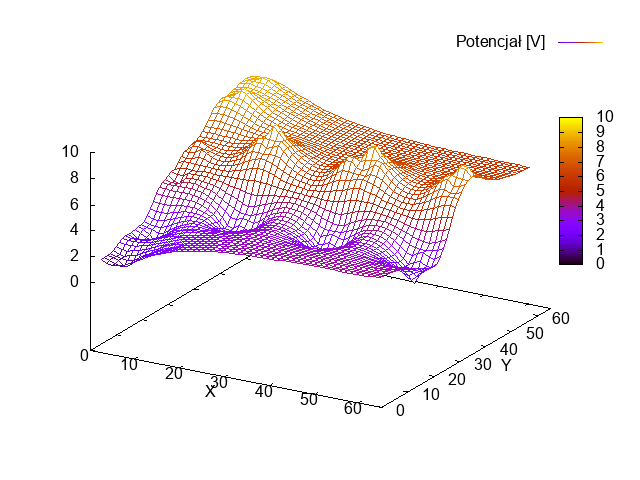
\includegraphics[width=18cm, height=16cm]{plotp}
\caption{Przybliżenie potencjału pola wewnątrz kondensatora}
\end{figure}

\subsection{Wizualizacja wektorów natężenia pola}

\begin{figure}[h]
\centering
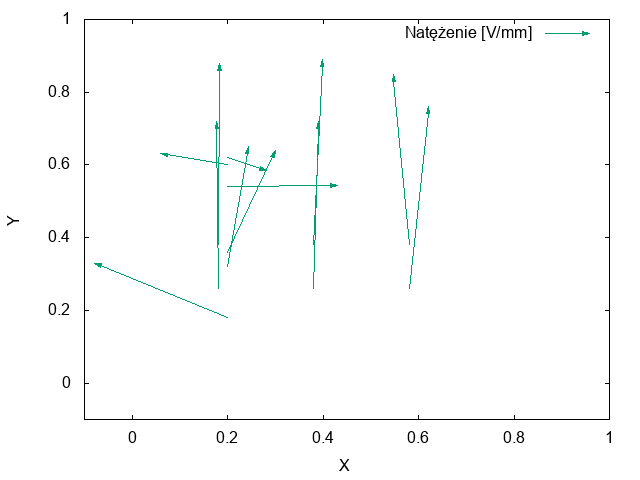
\includegraphics[width=18cm, height=16cm]{plotw}
\caption{Przybliżenie natężenia w postaci wektorów pola wewnątrz kondensatora}
\end{figure}

\section{Bibliografia}

\begingroup
\renewcommand{\section}[2]{}%
\begin{thebibliography}{}
\bibitem{instrukcja} \url{http://www.fis.agh.edu.pl/~pracownia_fizyczna/cwiczenia/31_wykon.pdf}
\bibitem{pe} \url{https://pl.wikipedia.org/wiki/Pole_elektryczne}
\bibitem{pote} \url{https://pl.wikipedia.org/wiki/Potencja%C5%82_elektryczny}
\bibitem{npe} \url{https://pl.wikipedia.org/wiki/Nat%C4%99%C5%BCenie_pola_elektrycznego}
\bibitem{konder} \url{https://pl.wikipedia.org/wiki/Kondensator}
\end{thebibliography}
\endgroup

\end{justify}

\end{document}